\chapter{Tijddilatatie en lengtecontractie}
\vspace{-1cm}\begin{flushright}
{\it `Its not that I am smart, \\it's just that I stay with the problem longer'}\\ A. Einstein
\end{flushright}

We hebben gezien dat Einstein in 1905 een rigoureuze stap zette 
door te postuleren dat er een relativiteitsprincipe moest bestaan dat zowel gold voor
mechanica als voor elektromagnetisme. De twee postulaten waarop de speciale relativiteitstheorie berusten zijn, zoals we eerder zagen
\begin{enumerate}
\item \underline{Het relativiteitsprincipe}\\ De natuurwetten en de
resultaten van alle experimenten uitgevoerd in een zeker
referentiestelsel zijn onafhankelijk van de translatiebeweging van het
systeem\footnote{We gebruiken de woorden referentiestelsel en
co\"{o}rdinatenstelsel door elkaar. De hier bedoelde equivalente
co\"{o}rdinatenstelsels worden ook wel inertiaalstelsels genoemd: dat
zijn dus referentiestelsels waarin dezelfde krachten werken,
c.q. `waarop' geen krachten werken, cf~\ref{v:galilei3}}.  In de
woorden van Einstein: als co\"{o}rdinatenstelsel $S^{'}$ met constante
snelheid rechtlijnig beweegt t.o.v. co\"{o}rdinatenstelsel $S$ dan
verlopen natuurkundige verschijnselen t.o.v. $S^{'}$ volgens precies
dezelfde natuurwetten als t.o.v. $S$.
\item \underline{Constantheid van de lichtsnelheid}\\ De lichtsnelheid
is eindig en {\sl on}afhankelijk van de bewegingstoestand van de lichtbron.
Het is de limietsnelheid voor natuurkundige objecten (in dit tweede
postulaat wordt impliciet aangenomen dat de lichtsnelheid als
fundamentele natuurconstante een universele rol speelt en niet alleen
van belang is voor verschijnselen waar licht bij betrokken is). Met
andere woorden: de lichtsnelheid heeft in ieder inertiaalstelsel
dezelfde waarde.

\end{enumerate}

\section{Synchroniseren van de tijd}
We hebben gezien dat alle beweging in de Newtonse
natuurkunde gebaseerd was op de grondgedachte: het bestaan van een
universele tijd. Maar we zagen dat dit niet langer houdbaar is, en
Einstein voegt toe ``de rechtvaardiging van een natuurkundig concept
is alleen mogelijke in duidelijke relatie met observaties''. 

Hoe meten we tijd? We kunnen de tijd meten aan de hand van een wekker,
een stopwatch, de rotatie van de aarde, de hartslag, etc. We noemen
dit in algemene zin een `klok'. En als we tijd meten, doen we dit altijd 
aan de hand van gelijktijdige gebeurtenissen. Bijvoorbeeld, als we zeggen
dat een trein om 7 uur op het station arriveert, bedoelen we: ``het
moment dat de kleine wijzer van mijn horloge op de 7 staat, 
en het arriveren van de trein, zijn twee gelijktijdige gebeurtenissen''. 

Dit klink triviaal, maar Einstein voorzag het volgende probleem.  Met
een klok kunnen we de snelheid van een voorwerp meten. Daartoe bepalen
we de plaats $\vec{r}_1$ van het voorwerp op tijdstip $t_1$ en de
plaats $\vec{r}_2$ op tijdstip $t_2$. Hiermee wordt de snelheid
\[
v = \frac{\vec{r}_2-\vec{r}_1}{t_2-t_1}.
\]
Maar dit betekent, gezien het bovenstaande, dat we gebruik moeten
maken van het aflezen van de tijd $t_1$ van een klok, op het moment
dat het lichaam op plaats $\vec{r}_1$ passeert, en gebruik maken van
een {\it andere} klok op plaats $\vec{r}_2$ om tijdstip $t_2$ te lezen
wanneer het lichaam in $\vec{r}_2$ arriveert. En welke klok we ook
gebruiken, onze meting van snelheid is zonder betekenis als we niet
zeggen wat we bedoelen met {\it dezelfde} tijd op twee verschillende
locaties. Als we informatie met oneindige snelheid konden versturen,
zou dit geen probleem opleveren. Maar dit is niet het geval; we kunnen
klokken niet beter synchroniseren dan met behulp van de snelheid van
het licht. 

Hoe kan dit synchroniseren in zijn werk gaan? We kunnen twee klokken
plaatsen, een op plaats $r_1$ en de ander op plaats $r_2$. We hebben
hiermee een `tijd op plaats $r_1$', en een `tijd op plaats $r_2$'
gedefini\"eerd. Om een {\it gemeenschappelijke} tijd voor $r_1$ en $r_2$
teweeg te brengen, kunnen we stellen dat de tijd voor een lichtsignaal
om van $r_1$ naar $r_2$ te komen, gelijk is aan die om van $r_2$ terug
naar $r_1$ te komen; zie het tweede postulaat. Nu kunnen we eenvoudig
een spiegel in $r_2$ zetten, en een lichtsignaal vanuit $r_1$ sturen
naar $r_2$, welke gereflecteerd wordt en weer terug komt in
$r_1$. Noem deze tijdsduur $t_0$, en we kunnen {\it defini\"eren} dat
het signaal in $r_2$ aankwam op tijdstip $t_0/2$.  Hiermee is de klok
op plaats $r_2$ gesynchroniseerd met de klok op plaats $r_1$. Dit
kunnen we voor een heel aantal klokken op elke plaats $r_i$ doen, en
zo klokken op elke willekeurige plaats synchroniseren.

\section{Relativiteit van gelijktijdigheid}
De consequentie van Einsteins manier om klokken  te synchroniseren op
verschillende plaatsen is dat {\it gelijktijdigheid} een relatief
begrip wordt, en niet langer absoluut geldig is. Dit kun je zien aan
hand van het volgende voorbeeld.

Stel je hiervoor een lange trein voor, met lengte $L$. Helemaal aan de
kop van de trein, en helemaal aan het einde van de trein, staan twee
klokken die de tijd meten. Een waarnemer die precies midden in de
trein staat, stuurt een lichtflits uit die zowel naar de kop als naar
het einde van de trein gaat. Omdat de lichtsnelheid naar beide kanten
gelijk is, zal deze waarnemer op de trein zeggen dat de klok op de
kop van de trein {\it tegelijkertijd} met de klok aan het einde van de
trein het licht signaal ontvangt. De waarnemer op de trein
zal dus concluderen dat de ontvangst van de lichtflits aan beide zijden van
de trein een {\it gelijktijdige}  gebeurtenis is.

Maar hoe vergaat het de waarnemer op het perron die de trein voorbij
ziet komen? Laten we aannemen dat het midden van de trein net 
langskomt als de lichtflits verstuurd wordt. Omdat de trein rijdt  zal
de flits naar de voorkant van de trein een iets langere
weg moeten afleggen. Dit omdat de trein een stukje verder rijdt gedurende
de tijd dat het licht nodig heeft om naar de klok aan de kop van de
trein te komen. Omgekeerd hoeft het licht een iets kortere weg af te
leggen om het einde van de trein te bereiken, omdat het einde van de
trein iets naar de waarnemer op het perron is toegekomen gedurende de
tijd die het licht nodig heeft om te reizen. Ook voor deze waarnemer
is de snelheid van het licht constant (tweede postulaat!), en hij komt
tot een andere conclusie. Voor hem bereikt de lichtflits het einde
van de trein {\it eerder} dan het licht de kop van de trein bereikt!
Voor hem zijn dit dus geen gelijktijdige gebeurtenissen. Met andere
woorden, dit `gedachtenexperiment' laat zien dat gelijktijdigheid
afhangt van de keuze van het inertiaalsysteem.
Overigens, om een
echt meetbaar verschil te geven met de waarnemer {\it op} de trein,
moet de trein natuurlijk wel met erg hoge snelheid langs het perron razen!

\section{Tijddilatatie} \label{s:lichtklok}
Stel twee waarnemers voor, Dirk (D) en Erika (E), die ten opzichte van
elkaar bewegen in twee ruimteschepen.  D meet de snelheid $v$ van E
ten opzichte van zijn ruststelsel. Als gevolg van de symmetrie van
deze situatie zal ook E een snelheid $v$ meten van de snelheid van D,
ten opzichte van haar ruststelsel. Als dit niet direct duidelijk is, bedenk dan dat 
in dit voorbeeld D en E volledig inwisselbaar zijn. Als D en E  niet dezelfde snelheid zouden meten, zou een van beide in een `speciaal' co\"ordinatenstelsel zitten, en dit is precies in tegenspraak met de postulaten van de relativiteitstheorie.

\begin{figure}[ht]
\centering
%\includegraphics[width=.5\textwidth]{syllabus.pictures/Lichtklok}
\epsfig{file=Lichtklok.pdf, width=0.5\textwidth}
\caption{{\sl Schematische tekening van een lichtklok. De lengte die het licht aflegt tussen lamp en detector is 1 m.}}
\label{f:lichtklok}
\end{figure}

Stel nu voor dat D en E beide een zeer bijzondere klok bij zich
hebben. Deze `licht-klokken' bestaan eenvoudigweg uit een lampje, een
spiegel, een fotodetector en wat elektronica. De fotodetector zit vlak
naast het lampje en de spiegel bevindt zich op 0.5 m hoogte, zie
figuur~\ref{f:lichtklok}. Als de klok gestart wordt gaat het lampje
eventjes aan, een lichtflits kaatst via de spiegel in de
fotodetector. Wanneer de fotodetector het licht registreert, geeft het
een signaal aan het lampje om onmiddellijk een nieuwe lichtflits uit te
zenden. Zo tikken de lichtflitsen met een regelmaat van $1/c \sim 3.3
\times 10^{-9}$ s, oftewel elke 3.3 ns een tik. De lichtsnelheid is
hetzelfde voor alle waarnemers, dus $c$ is hier een conversiefactor
tussen tijd en afstand. Deze lichtklok tikt de tijd in
meters\footnote{Het ISO (International Standard Organization)
defini\"eert zo de meter in termen van seconden. De lichtsnelheid
wordt daarbij {\it gedefini\"eerd} met een waarde $c=2.99792458 \times
10^8$ m s$^{-1}$.}.

Stel nu dat D de klok rechtop houdt, zodanig dat het licht loodrecht op zijn
bewegingsrichting ten opzichte van E kaatst. We hebben gezien dat D zijn klok tikt
met intervallen van 3.3 ns., maar wat ziet E? Merk op dat D beweegt
met een snelheid $v$ ten opzichte van E, dus in het ruststelsel van E
maakt het licht geen echte rondgang. Gedurende de reis van het licht
omhoog naar de spiegel en terug legt D een afstand af in de
loodrechte richting; het pad van het licht wordt een zig-zag, en is
langer dan het rechte op-neer pad bij een stilstaande klok, zie figuur~\ref{f:lichtklok2}.

\begin{figure}[ht]
\centering
%\includegraphics[width=.5\textwidth]{syllabus.pictures/Lichtklok2}
\epsfig{file=Lichtklok2.pdf, width=0.5\textwidth}
\caption{{\sl Het traject van het licht in de klok van waarnemer D zoals
geobserveerd door D (a) en E (b). Merk op dat het traject langer is in
het stelsel van E, en dus meet E een langer tijdsinterval $t'$.}}
\label{f:lichtklok2}
\end{figure}

Toch meten waarnemers dezelfde lichtsnelheid $c$ (het
relativiteitsprincipe!), en moeten we concluderen dat E een groter
tijdsinterval $\Delta t'$ tussen twee tikken meet dan waarnemer D\footnote{Alle grootheden die E meet worden met een accent
weergegeven, de grootheden die D meet zonder accent.}.
 Wat is het verschil tussen $\Delta t$ en $\Delta t'$?

In het stelsel van E, in een tijd $\Delta t'$, beweegt D het stuk
$\Delta x'=v \Delta t'$ naar voren, en legt het licht een afstand
$\Delta l' = c\Delta t'$ af. Volgens Pythagoras is $(\Delta l')^2
=(\Delta x')^2 +(\Delta y')^2$ waarbij $\Delta y'$ de lengte
van het traject in de $y$ richting is.  We zullen later aantonen dat $\Delta y'
= \Delta y$, en is dus 1 m. Omdat in het stelsel van D geldt $\Delta y= \Delta l = c \Delta t$ vinden we
\begin{equation}\label{e:timedil}
\Delta t' = \frac{\Delta t}{\sqrt{1-\frac{v^2}{c^2}}}
\end{equation}
De tijdsintervallen tussen de tikken van de klok van D zijn groter
zoals gemeten door E dan zoals gemeten door D. Dit effect heet {\it
tijddilatatie}. Bewegende klokken lopen langzamer.

In de literatuur wordt vaak de volgende notatie gebruikt. De dimensieloze grootheid $\beta$ staat voor de snelheid, 
\begin{equation}
\beta = \frac{v}{c},
\end{equation}
en omdat niets sneller kan gaan dan de lichtsnelheid $c$, geldt $-1 \leq \beta \leq 1$. De {\it Lorentzfactor} $\gamma$ is gedefinieerd als
\begin{equation}
\gamma = \frac{1}{\sqrt{1-\frac{v^{2}}{c^{2}}}} = \frac{1}{\sqrt{1-\beta^2}}\label{f:gamma}
\end{equation}
Voor deze factor geldt $\gamma \geq 1$. Met deze nieuwe symbolen wordt formule~\ref{e:timedil} geschreven als $\Delta t' = \gamma \Delta t$. 

We hebben nu gevonden dat `bewegende klokken langzaam lopen'. Een punt
van kritiek zou kunnen zijn dat dit alleen is aangetoond voor deze
merkwaardige lichtklokken. Toch kunnen we laten zien dat {\it alle}
klokken onderhevig zijn aan dit dilatatie effect. Stel namelijk voor
dat, naast de lichtklok, waarnemer D ook nog een horloge of een ander
mechanisme heeft om de tijd te meten dat elke 3.3 ns tikt. En stel
voor (hetgeen onjuist is!) dat dit horloge geen tijd-dilatatie effect
ondergaat; dat wil zeggen, stel voor dat E het horloge elke 3.3 ns
ziet tikken ongeacht de snelheid van D. Wanneer D stilstaat ten
opzichte van E tikken het horloge en de lichtklok met dezelfde
snelheid, maar wanneer D met hoge snelheid beweegt beginnen ze
ongelijk te tikken omdat (zoals we veronderstelden) de \'e\'en
tijd-dilatatie heeft en de ander niet. Maar dan kan D uit de relatieve
tik-snelheden van het horloge en de lichtklok achterhalen wat zijn
snelheid is, en zo schendt hij het relativiteitsprincipe. Het is niet
mogelijk de klokken gelijk te laten lopen voor waarnemer D, en ze
ongelijk te laten lopen voor waarnemer E.

Men kan opmerken dat het relativiteitsprincipe al is
geschonden. Immers, als D en E in deze symmetrische situatie zitten,
hoe kan het dan dat E langere tijdsintervallen meet dan D? Welke
intervallen meet D ten opzichte van E? Nu moeten we voorzichtig zijn:
E meet langere intervallen voor de klok van D dan D zelf meet. Door
het relativiteitsprincipe moet het daarom zijn dat D {\it ook} grotere
tijdsduur intervallen meet voor een klok in het ruimtestation van E,
dan E zelf meet. En dit is juist, uiteindelijk kunnen we D en E in de
hele argumentatie verwisselen. Dit is het fundamentele
tegen-intu\"itive karakter van de relativiteitstheorie. Hoe kan het
dat beide waarnemers langzamere tijdsintervallen meten van elkaars
klokken? Feit blijkt dat er helemaal geen tegenspraak in deze bewering
zit zodra we het concept van `absolute tijd' voor alle waarnemers,
waar Newton zo aan hechtte, opgeven.

\subsection{Observatie van tijddilatatie}
In de vorige paragraaf, zoals in de rest van dit college, is het
belangrijk een verschil te maken tussen wat een ideale waarnemer {\it
observeert} en wat een ideale waarnemer {\it ziet}. `Observeren' staat
voor `het meten van echte effecten met de juiste experimentele
technieken', terwijl `zien' is gereserveerd voor schijnbare effecten,
of fenomenen die gerelateerd zijn aan het feit dat we vanuit een
specifiek gezichtspunt kijken met een specifiek paar ogen.

Hoewel E {\it observeert} dat de klok van D langzaam loopt, {\it ziet}
zij wellicht iets heel anders. De tijds intervallen tussen de tikken
van de klok van D die zij ziet, hangen af van het tijddilatatie effect
{\it en} de verandering van de afstand die het licht moet afleggen om
naar E te komen. Deze afstand verandert omdat D beweegt ten opzichte
van E, zie figuur~\ref{f:tijdpad}.

\begin{figure}[ht]
\centering
%\includegraphics[width=.5\textwidth]{syllabus.pictures/Tijdpad}
\epsfig{file=Tijdpad.pdf, width=0.5\textwidth}
\caption{{\sl Observeren van tijddilatatie. Omdat D beweegt ten opzichte
van E, leggen de lichtflitsen ($F_1$ tot $F_4$) van zijn klok
verschillende afstanden ($S_1$ tot $S_4$) af om waarnemer E te
bereiken. Dus de tijd om E te bereiken is verschillend voor de
lichtflitsen. E moet hiervoor corrigeren voordat zij een uitspraak kan
doen over tijddilatatie. Pas nadat deze correcties zijn gemaakt
observeert E de voorspelde tijddilatatie.}}
\label{f:tijdpad}
\end{figure}


U zult ontdekken dat het tijdsinterval tussen twee tikken veel langer
is dan wat tijddilatatie voorspeld, omdat
opeenvolgende flitsen van verder en verder weg moeten komen. Dit effect heet
{\it Doppler-verschuiving} en zal verder in het college behandeld
worden.

\section{Lengtecontractie} \label{s:contractie}
Stel nu dat er twee planeten zijn, A en B, beide in rust ten opzichte van  waarnemer E.
Waarnemer D maakt een reis van A naar B terwijl waarnemer E stilstaat bij een planeet.
Gedurende de reis van D ziet waarnemer E dat er 100 tikken verstrijken op de klok van D.
 
Dan moet D ook zelf 100 tikken zien verstrijken gedurende deze
reis. Immers, het is mogelijk de klok bijvoorbeeld een gaatje te laten
prikken in een kaart elke keer dat het tikt. D kan het prikken laten
beginnen bij planeet A en laten eindigen bij planeet B, en er moeten
dan een bepaald aantal prikken in de kaart zitten. D en E moeten met
elkaar overeenstemmen hoeveel gaatjes er in de kaart zitten; zij
kunnen immers altijd na de reis bij elkaar komen en de gaatjes tellen.

Behalve het aantal gaatjes, zijn ze het ook eens over hun onderlinge
snelheid (ze moeten wel: hun situatie is volledig inwisselbaar - dit
argument is eerder gemaakt). Echter, waar ze het niet met elkaar over
eens zijn is de snelheid waarmee elkaars klokken tikken. E bepaalt de
afstand tussen de planeten A en B als $l'=100 v \Delta t'$. Echter, 
D bepaalt de afstand als $100 v \Delta t = l'/\gamma$. Omdat $\gamma > 1$ meet
D een {\it kortere} afstand dan E.  D beweegt ten opzichte van de
planeten A en B, terwijl E stil staat ten opzichte van deze planeten.
In feite kunnen de planeten A en B gezien worden als de eind-punten
van een heel lange meetlat die waarnemer E vasthoudt; een meetlat die
beweegt ten opzichte van D.  We concluderen dat een bewegende meetlat
korter wordt; dit effect heet lengtecontractie oftewel 
{\it Lorentzcontractie}.

Het is eenvoudig aan te tonen dat deze Lorentzcontractie alleen
optreedt in de richting parallel aan de bewegingsrichting. Immers,
stel dat E en D beide een holle pijp van heel dun materiaal hebben, beide met exact dezelfde diameter, zodat de pijpen niet in elkaar geschoven kunnen worden.
Stel nu dat de ori\"entatie van de pijpen  parallel aan hun onderlinge
bewegingsrichting is. Als we nu aannemen (wat niet juist is!) dat
de diameter van E's pijp anders wordt in het co\"ordinatenstelsel van
D, zou de pijp van D om die van E heen passen. Maar in de omgekeerde situatie zou dan de pijp van D kleiner moeten worden in het co\"ordinatenstelsel van E!
Hier is een contradictie, en we concluderen dat de diameter van de
pijp niet verandert bij beweging loodrecht op deze diameter.

Merk op dat we eerder bij de lichtklok hadden aangenomen dat de
lengte $y$ loodrecht op de beweging niet veranderd van
referentiesysteem naar referentiesysteem. Dit hebben we nu aangetoond.

\section{Niet-relativistische limiet}
We zien dat wanneer $v \ll c$ de Lorentzfactor 
$\gamma = \sqrt{\frac{1}{1-\beta^2}}$ vrijwel gelijk is 
aan $1$ en relativistische effecten geen rol van betekenis spelen (zie Figuur \ref{fig:gammagraf}).
Een voertuig met een lengte van $4$ m dat met $100$ km/uur beweegt, is
$2\cdot 10^{-18}$ m korter dan  wanneer het in rust is.
Dat is $0.2 \%$  van de diameter van een proton...

\begin{figure}[t]
	\centering
%		\includegraphics[width=1.00\textwidth]{syllabus.pictures/gammagraf}
		\epsfig{file=gammagraf.pdf, width=\textwidth}
	\caption{{\sl Grafiek van $\gamma$ uitgezet tegen v/c. Duidelijk te zien is de asymptoot bij de lichtsnelheid, v/c = 1: daar wordt $\gamma \rightarrow \infty$. Tevens is het gedrag bij zeer lage snelheid (v/c $\approx 0$) duidelijk zichtbaar: $\gamma \approx 1$, het klassieke domein.}}
	\label{fig:gammagraf}
\end{figure}


\section{Kosmische stralen}
Onze atmosfeer wordt voortdurend gebombardeerd door kosmische straling.
Kosmische stralen zijn deeltjes van vaak hoge energie die ons uit het heelal 
bereiken, o.a. (in feite voornamelijk) protonen\footnote{Oorsprong, energiespectrum en samenstelling van kosmische stralen 
vormen interessante, nog lang niet opgehelderde onderwerpen van 
wetenschappelijk onderzoek.}. Deze protonen raken stikstof- of zuurstofkernen op grote hoogte, tientallen 
kilometers boven het aardoppervlak, in de bovenste lagen van de atmosfeer. We weten dat bij die botsingen o.a. muonen (symbool voor een muon: $\mu$)
geproduceerd worden. We weten\footnote{Vakgebied : hoge-energiefysica}
ook dat muonen in rust in ons laboratorium een (gemiddelde) levensduur 
hebben van $\tau = 2,2\ \mu$s $= 2,2\cdot  10^{-6}$s.
Volgens de niet-relativistische formule zou een muon, zelfs als het met de 
lichtsnelheid $c$ bewoog, slechts (gemiddeld) een 
afstand $c\tau = 659$ m afleggen.
We nemen de muonen echter op het aardoppervlak waar, dus ze reizen 
pakweg $30$ km.
Dus hun levensduur, gezien door een waarnemer op aarde, is een factor 
$30.000/659$ groter dan de levensduur in het rustsysteem van het muon.
Dus: $\gamma = 30.000/659 = 45.5$ waaruit volgt $v = 0,9998$ c.
De muonen reizen dus vrijwel met de lichtsnelheid en leven dankzij de 
tijddilatatie lang genoeg om de $30$ km te overbruggen.

\section{Tweelingparadox}
De resultaten van de relativiteitstheorie kunnen aanleiding geven tot 
`tegenstellingen' die de theorie ter discussie stellen.
Het gaat hier dan om schijnbare tegenstellingen, paradoxen, die ons er 
alleen maar voor waarschuwen dat de theorie zorgvuldig en correct 
ge\"{i}nterpreteerd dient te worden.
Laten we als voorbeeld nemen: tijddilatatie, 
`bewegende klokken lopen langzamer'.\\
Vanuit $S$ zien we een met $S^{'}$ meebewegende klok langzamer lopen, 
vanuit $S^{'}$ zien we een in $S$ in rust zijnde klok langzamer lopen.\\
Dat lijkt in tegenspraak, wie heeft er nu gelijk, de waarnemer in $S$ of 
die in $S^{'}$?
Natuurlijk hebben ze allebei gelijk en is er geen tegenspraak.
Wanneer we twee klokken willen vergelijken moeten we dat in hetzelfde 
referentiestelsel op dezelfde plaats doen.\\
Indien we de klokken uit het voorbeeld vervangen door leden van een tweeling, 
waarvan er \'{e}\'{e}n op aarde blijft en de ander vertrekt in een ruimteschip 
dan doet zich dezelfde situatie voor: beide nemen waar dat de ander minder 
snel oud wordt en dat is volkomen in orde.
Het `probleem' ontstaat wanneer de ruimtereiziger besluit om huiswaarts te 
keren om de andere helft van de tweeling te bezoeken.
Dan blijkt de ruimtereiziger wel degelijk jonger te zijn.
(Dit is geverifi\"{e}erd met aan boord van vliegtuigen vervoerde nauwkeurige 
klokken.)
Maar: het omkeren van de ruimtereiziger is niet te beschrijven als een 
eenvoudige Lorentztransformatie, anders gezegd: het rustsysteem van de 
ruimtereiziger, $S^{'}$, is geen inertiaalsysteem.
Systeem  $S$ 
is dat wel en daarom is het correct de situatie vanuit $S$ te beschrijven 
en in $S$ is de ruimtereiziger inderdaad langzamer verouderd dan de 
achterblijver.



